\documentclass[../thesis.tex]{subfiles}

\begin{document}

\appendix

\chapter{Data Description}
\label{chap:data_desc}

\noindent In this appendix we present a descriptive overview of the data used in this thesis. This includes: an overview and explanation of the variables used (\ref{sec:variables}), the \texttt{R}-packages (\ref{sec:r_pack}) used and some relevant plots (\ref{sec:rel_plots}) to support the finding in the thesis. The source code used to produce the relevant plots can be found in appendix (\ref{chap:souce_code}).  

\section{Variables}
\label{sec:variables}

\section{\texttt{R}-packages}
\label{sec:r_pack}

\section{Descriptive Statistics}
\label{sec:desc_stat}


\begin{scriptsize}
\begin{tabularx}{\textwidth}{P{3cm}rrrrrrrrrr}
\caption{Patient characteristics: HFpEF}\label{tab:desc_stat_HFpEF_variables}\\
\toprule
\textbf{Variable} & $n$ & \#Na & Min & Max & $\bar{x}$ & $\widetilde{x}$ & $s$ & $q_1$ & $q_3$ \\ 
\midrule
\endfirsthead
\caption*{\textbf{Table \ref{tab:desc_stat_HFpEF_variables}:} Patient characteristics: HFpEF (\textit{continued})}\\
\toprule
 \textbf{Variable} & $n$ & \#Na & Min & Max & $\bar{x}$ & $\widetilde{x}$ & $s$ & $q_1$ & $q_3$ \\ 
\midrule
\endhead
\multicolumn{10}{c}{PANEL II: Demographics}\\
\midrule
  age & 193 &   0 &  29.0 &   100.8 &   76.3 &   78.9 &   12.1 &  69.5 &   85.4 \\ 
  gender & 193 &   0 &   0.0 &     1.0 &    0.6 &    1.0 &    0.5 &   0.0 &    1.0 \\ 
  white & 193 &   0 &   0.0 &     1.0 &    0.7 &    1.0 &    0.5 &   0.0 &    1.0 \\ 
  asian & 193 &   0 &   0.0 &     1.0 &    0.1 &    0.0 &    0.2 &   0.0 &    0.0 \\ 
  black & 193 &   0 &   0.0 &     1.0 &    0.3 &    0.0 &    0.4 &   0.0 &    1.0 \\
\midrule
\multicolumn{10}{c}{PANEL III: Admission symptoms}\\
\midrule
  breathless & 185 &   8 &   0.0 &     1.0 &    0.8 &    1.0 &    0.4 &   1.0 &    1.0 \\ 
\midrule
\multicolumn{10}{c}{PANEL IV: Admission signs}\\
\midrule
  sbp & 182 &  11 &  55.0 &   242.0 &  146.9 &  145.0 &   31.7 & 125.0 &  167.0 \\ 
  dbp & 183 &  10 &  25.0 &   195.0 &   80.5 &   80.0 &   22.1 &  67.0 &   89.0 \\ 
  admissionwgt & 160 &  33 &  41.5 &   158.0 &   78.9 &   76.7 &   23.3 &  60.1 &   93.9 \\ 
  bp & 192 &   1 &   0.0 &     1.0 &    0.8 &    1.0 &    0.4 &   1.0 &    1.0 \\ 
  bmiadmission & 148 &  45 &  16.8 &   107.1 &   30.7 &   29.3 &   10.5 &  23.6 &   35.4 \\ 
  pulse & 182 &  11 &  44.0 &   211.0 &   84.7 &   83.0 &   22.1 &  70.0 &   95.0 \\
\midrule
\multicolumn{10}{c}{PANEL V: Risk factors}\\
\midrule
  a-fib & 189 &   4 &   0.0 &     1.0 &    0.5 &    0.0 &    0.5 &   0.0 &    1.0 \\ 
  copdasthma & 190 &   3 &   0.0 &     1.0 &    0.4 &    0.0 &    0.5 &   0.0 &    1.0 \\ 
  irondef &  69 & 124 &   0.0 &     1.0 &    0.6 &    1.0 &    0.5 &   0.0 &    1.0 \\ 
  dm & 188 &   5 &   0.0 &     1.0 &    0.5 &    1.0 &    0.5 &   0.0 &    1.0 \\ 
  obesity & 185 &   8 &   0.0 &     1.0 &    0.5 &    1.0 &    0.5 &   0.0 &    1.0 \\ 
  copdasthma.1 & 190 &   3 &   0.0 &     1.0 &    0.4 &    0.0 &    0.5 &   0.0 &    1.0 \\ 
  ihd & 186 &   7 &   0.0 &     1.0 &    0.4 &    0.0 &    0.5 &   0.0 &    1.0 \\ 
\midrule
\multicolumn{10}{c}{PANEL VI: Comorbidities}\\
\midrule
  comorbidities & 193 &   0 &   0.0 &     9.0 &    4.2 &    4.0 &    1.8 &   3.0 &    5.0 \\ 
\midrule
\multicolumn{10}{c}{PANEL VII: Electrocardiography}\\
\midrule
  ecgqrsduration & 157 &  36 &  55.0 &   177.0 &  101.3 &   98.0 &   20.8 &  88.0 &  112.0 \\ 
  ecgqrsother & 193 &   0 &   0.0 &     1.0 &    0.0 &    0.0 &    0.2 &   0.0 &    0.0 \\ 
  ecgrate & 159 &  34 &  41.0 &   191.0 &   83.0 &   80.0 &   23.1 &  70.0 &   92.0 \\ 
  ecgrhythmother & 193 &   0 &   0.0 &     1.0 &    0.1 &    0.0 &    0.2 &   0.0 &    0.0 \\ 
  lvh & 169 &  24 &   0.0 &     1.0 &    0.1 &    0.0 &    0.3 &   0.0 &    0.0 \\ 
  normalecgqrs & 193 &   0 &   0.0 &     1.0 &    0.6 &    1.0 &    0.5 &   0.0 &    1.0 \\ 
  lbbb & 193 &   0 &   0.0 &     1.0 &    0.0 &    0.0 &    0.2 &   0.0 &    0.0 \\ 
  rbbb & 193 &   0 &   0.0 &     1.0 &    0.1 &    0.0 &    0.3 &   0.0 &    0.0 \\ 
  sr & 193 &   0 &   0.0 &     1.0 &    0.6 &    1.0 &    0.5 &   0.0 &    1.0 \\
\midrule
\multicolumn{10}{c}{PANEL VIII: Laboratory tests}\\
\midrule
  hb & 192 &   1 &  47.0 &   185.0 &  107.6 &  107.5 &   21.1 &  91.8 &  123.0 \\ 
  wbc & 192 &   1 &   2.9 &   209.4 &   10.2 &    7.6 &   15.8 &   6.0 &   10.5 \\ 
  tsat &  94 &  99 &   4.0 &    92.0 &   20.4 &   18.0 &   13.8 &  11.0 &   24.8 \\ 
  plts & 192 &   1 &  51.0 &   497.0 &  229.4 &  217.0 &   89.5 & 163.0 &  284.2 \\ 
  pcv & 193 &   0 &   0.2 &     0.6 &    0.3 &    0.3 &    0.1 &   0.3 &    0.4 \\ 
  ferritin &  71 & 122 &   9.0 &  2223.0 &  378.2 &  173.0 &  533.8 &  61.5 &  443.5 \\ 
  k & 189 &   4 &   2.4 &     8.7 &    4.4 &    4.4 &    0.6 &   4.1 &    4.7 \\ 
  ironlevels &  95 &  98 &   2.0 &    23.0 &    8.6 &    7.0 &    4.8 &   5.0 &   11.0 \\ 
  chol & 190 &   3 &   0.0 &     1.0 &    0.5 &    1.0 &    0.5 &   0.0 &    1.0 \\ 
  ntprobnp & 193 &   0 &  81.0 & 70000.0 & 5047.3 & 2217.0 & 8487.4 & 997.0 & 5305.0 \\ 
  gfr & 193 &   0 &   3.0 &   221.0 &   54.1 &   47.0 &   31.1 &  32.0 &   72.0 \\ 
  mcv & 193 &   0 &  57.0 &   117.0 &   88.8 &   89.0 &    8.9 &  85.0 &   94.0 \\ 
  na & 193 &   0 & 110.0 &   148.0 &  138.2 &  139.0 &    4.9 & 136.0 &  141.0 \\
\midrule
\multicolumn{10}{c}{PANEL IX: Echocardiography}\\
\midrule
  lvef & 191 &   2 &  50.0 &    72.5 &   57.1 &   57.5 &    4.5 &  55.0 &   60.0 \\ 
  ewave & 174 &  19 &   0.4 &     1.6 &    0.9 &    0.9 &    0.3 &   0.7 &    1.1 \\ 
  pasp & 122 &  71 &  14.0 &    85.0 &   43.5 &   42.5 &   14.2 &  34.0 &   51.8 \\ 
  ee & 152 &  41 &   2.0 &    37.0 &   13.4 &   12.5 &    5.8 &   9.0 &   16.0 \\ 
  mr & 193 &   0 &   0.0 &     2.0 &    0.5 &    0.0 &    0.7 &   0.0 &    1.0 \\ 
  tr & 193 &   0 &   0.0 &     3.0 &    0.9 &    1.0 &    0.8 &   0.0 &    1.0 \\ 
  as & 193 &   0 &   0.0 &     2.0 &    0.1 &    0.0 &    0.3 &   0.0 &    0.0 \\ 
  ai & 193 &   0 &   0.0 &     2.0 &    0.2 &    0.0 &    0.5 &   0.0 &    0.0 \\ 
  rvfunction & 192 &   1 &   0.0 &     4.0 &    0.6 &    0.0 &    1.2 &   0.0 &    0.2 \\ 
  af & 193 &   0 &   0.0 &     1.0 &    0.2 &    0.0 &    0.4 &   0.0 &    0.0 \\ 
\midrule
\multicolumn{10}{c}{PANEL X: Outcomes}\\
\midrule
  timetohfadm &  69 & 124 &   3.8 &   718.8 &  192.5 &  122.7 &  197.8 &  33.0 &  270.0 \\ 
  hfhospitalisation & 193 &   0 &   0.0 &     1.0 &    0.4 &    0.0 &    0.5 &   0.0 &    1.0 \\ 
  los & 171 &  22 &   1.0 &   372.0 &   15.8 &    8.0 &   31.3 &   4.0 &   19.0 \\ 
\midrule
\end{tabularx}
\end{scriptsize}


\begin{scriptsize}
\begin{tabularx}{\textwidth}{P{3cm}RRRRRRRRRR}
\caption{Patient characteristics: HFmrEF}\label{tab:desc_stat_HFmrEF_variables}\\
\toprule
\textbf{Variable}\parnote{\scriptsize Note: $n$ - number of observations, \#Na - number of missing data, Min - minimal, Max - maximal,  $\bar{x}$ - arithmetic mean, $\widetilde{x}$ - median, $s$ - standard deviation, $q_1$ - first quartile and $q_3$ - third quartile.} & $n$ & \# Na & Min & Max & $\bar{x}$ & $\widetilde{x}$ & $s$ & $q_1$ & $q_3$ \\ 
\midrule
\endfirsthead
\caption*{\textbf{Table \ref{tab:desc_stat_HFmrEF_variables}:} Patient characteristics: HFmrEF (\textit{continued})}\\
\toprule
 \textbf{Variable} & $n$ & \#Na & Min & Max & $\bar{x}$ & $\widetilde{x}$ & $s$ & $q_1$ & $q_3$ \\ 
\midrule
\endhead
\multicolumn{10}{c}{PANEL I: Identification}\\
\midrule
patientid & 182 &   0 &     1.0 &    193.0 &    96.9 &    97.5 &    56.6 &    47.2 &   146.5 \\ 
\midrule
\multicolumn{10}{c}{PANEL II: Demographics}\\
\midrule
  gender & 182 &   0 &  0.0 &      1.0 &    0.4 &    0.0 &     0.5 &    0.0 &    1.0 \\ 
  white & 182 &   0 &  0.0 &      1.0 &    0.7 &    1.0 &     0.5 &    0.0 &    1.0 \\ 
  asian & 182 &   0 &  0.0 &      1.0 &    0.1 &    0.0 &     0.3 &    0.0 &    0.0 \\ 
  black & 182 &   0 &  0.0 &      1.0 &    0.2 &    0.0 &     0.4 &    0.0 &    0.0 \\
\midrule
\multicolumn{10}{c}{PANEL III: Admission symptoms}\\
\midrule
  breathless &  55 & 127 &  0.0 &      3.0 &    2.4 &    3.0 &     1.0 &    2.0 &    3.0 \\  
\midrule
\multicolumn{10}{c}{PANEL IV: Admission signs}\\
\midrule
  sbp &  98 &  84 & 86.0 &    242.0 &  132.6 &  126.5 &    27.7 &  114.2 &  147.8 \\ 
  dbp &  95 &  87 & 45.0 &    591.0 &   80.2 &   72.0 &    55.7 &   62.0 &   85.0 \\ 
  admissionwgt &  51 & 131 & 21.0 &    134.9 &   80.6 &   80.6 &    21.8 &   66.7 &   96.4 \\ 
  bp & 182 &   0 &  0.0 &      1.0 &    0.7 &    1.0 &     0.5 &    0.0 &    1.0 \\ 
  bmiadmission &   4 & 178 & 18.7 &     36.1 &   26.0 &   24.7 &     8.0 &   20.2 &   30.5 \\ 
  pulse &  98 &  84 & 54.0 &    144.0 &   88.8 &   85.0 &    21.9 &   71.2 &  100.0 \\
\midrule
\multicolumn{10}{c}{PANEL V: Risk factors}\\
\midrule
  a-fib & 182 &   0 &  0.0 &      1.0 &    0.4 &    0.0 &     0.5 &    0.0 &    1.0 \\ 
  copdasthma & 181 &   1 &  0.0 &      1.0 &    0.3 &    0.0 &     0.5 &    0.0 &    1.0 \\ 
  irondef &  52 & 130 &  0.0 &      1.0 &    0.4 &    0.0 &     0.5 &    0.0 &    1.0 \\ 
  dm & 180 &   2 &  0.0 &      1.0 &    0.4 &    0.0 &     0.5 &    0.0 &    1.0 \\ 
  obesity &  53 & 129 &  0.0 &      1.0 &    0.5 &    1.0 &     0.5 &    0.0 &    1.0 \\ 
  ihd & 181 &   1 &  0.0 &      1.0 &    0.5 &    0.0 &     0.5 &    0.0 &    1.0 \\ 
\midrule
\multicolumn{10}{c}{PANEL VI: Comorbidities}\\
\midrule
  comorbidities & 182 &   0 &  0.0 &      7.0 &    3.2 &    3.0 &     1.7 &    2.0 &    4.0 \\ 
\midrule
\multicolumn{10}{c}{PANEL VII: Electrocardiography}\\
\midrule
  ecgqrsduration &  77 & 105 & 71.0 &    182.0 &  104.9 &   99.0 &    24.0 &   88.0 &  116.0 \\ 
  ecgqrsother & 182 &   0 &  0.0 &      1.0 &    0.1 &    0.0 &     0.2 &    0.0 &    0.0 \\ 
  ecgrate &  88 &  94 & 42.0 &    135.0 &   86.2 &   83.5 &    21.5 &   72.2 &   99.2 \\ 
  ecgrhythmother & 182 &   0 &  0.0 &      1.0 &    0.0 &    0.0 &     0.1 &    0.0 &    0.0 \\ 
  lvh & 180 &   2 &  0.0 &      3.0 &    0.6 &    0.0 &     0.8 &    0.0 &    1.0 \\ 
  normalecgqrs & 182 &   0 &  0.0 &      1.0 &    0.3 &    0.0 &     0.4 &    0.0 &    1.0 \\ 
  lbbb & 182 &   0 &  0.0 &      1.0 &    0.0 &    0.0 &     0.2 &    0.0 &    0.0 \\ 
  rbbb & 182 &   0 &  0.0 &      1.0 &    0.0 &    0.0 &     0.2 &    0.0 &    0.0 \\ 
  sr & 182 &   0 &  0.0 &      1.0 &    0.0 &    0.0 &     0.2 &    0.0 &    0.0 \\
\midrule
\multicolumn{10}{c}{PANEL VIII: Laboratory tests}\\
\midrule
  hb & 168 &  14 & 54.0 &    153.0 &  110.7 &  111.0 &    19.9 &   98.0 &  125.0 \\ 
  wbc & 166 &  16 &  1.5 &     39.2 &    8.3 &    7.6 &     4.2 &    5.9 &    9.4 \\ 
  tsat &  71 & 111 &  1.0 &     65.0 &   20.4 &   19.0 &    12.5 &   14.0 &   25.0 \\ 
  plts & 166 &  16 & 55.0 &    638.0 &  203.8 &  187.0 &    92.3 &  143.2 &  246.5 \\ 
  pcv & 166 &  16 &  0.2 &      0.5 &    0.3 &    0.3 &     0.1 &    0.3 &    0.4 \\ 
  ferritin &  54 & 128 & 17.0 &   3853.0 &  370.2 &  225.0 &   556.3 &  102.8 &  448.0 \\ 
  k & 165 &  17 &  3.0 &      6.1 &    4.4 &    4.4 &     0.6 &    4.0 &    4.8 \\ 
  ironlevels &  70 & 112 &  2.0 &     41.0 &    9.5 &    8.0 &     7.1 &    5.0 &   11.0 \\ 
  chol & 181 &   1 &  0.0 &      1.0 &    0.4 &    0.0 &     0.5 &    0.0 &    1.0 \\ 
  ntprobnp & 182 &   0 &  5.0 &  70000.0 & 9604.4 & 4063.5 & 14051.2 & 1886.5 & 9968.2 \\ 
  gfr & 167 &  15 &  3.0 &    400.0 &   53.5 &   47.0 &    39.8 &   31.0 &   68.5 \\ 
  mcv & 166 &  16 & 65.0 &    112.0 &   91.0 &   92.0 &     8.4 &   86.0 &   96.0 \\ 
  na & 168 &  14 &  4.7 &    155.0 &  137.5 &  139.0 &    11.5 &  136.0 &  141.0 \\
\midrule
\multicolumn{10}{c}{PANEL IX: Echocardiography}\\
\midrule
  lvef & 182 &   0 & 40.0 &     50.0 &   44.0 &   45.0 &     2.9 &   42.0 &   47.5 \\ 
  ewave & 139 &  43 &  0.3 &      5.0 &    0.9 &    0.9 &     0.5 &    0.7 &    1.0 \\ 
  pasp &  72 & 110 & 18.0 & 251520.0 & 3856.5 &   40.0 & 29625.6 &   32.0 &   53.2 \\ 
  ee &  88 &  94 &  3.0 &     43.0 &   14.9 &   13.5 &     7.3 &    9.0 &   19.2 \\ 
  mr & 159 &  23 &  0.0 &      3.0 &    0.8 &    1.0 &     0.8 &    0.0 &    1.0 \\ 
  tr & 157 &  25 &  0.0 &      3.0 &    0.9 &    1.0 &     0.9 &    0.0 &    1.0 \\ 
  as & 140 &  42 &  0.0 &      2.0 &    0.2 &    0.0 &     0.5 &    0.0 &    0.0 \\ 
  ai & 151 &  31 &  0.0 &      3.0 &    0.3 &    0.0 &     0.5 &    0.0 &    0.0 \\ 
  rvfunction & 146 &  36 &  0.0 &      6.0 &    1.2 &    0.0 &     2.0 &    0.0 &    1.0 \\ 
  af & 182 &   0 &  0.0 &      1.0 &    0.2 &    0.0 &     0.4 &    0.0 &    0.0 \\ 
\midrule
\multicolumn{10}{c}{PANEL X: Outcomes}\\
\midrule
  timetohfadm & 122 &  60 &  0.4 &    575.9 &   84.5 &   44.9 &   109.6 &   11.9 &  114.7 \\ 
  hfhospitalisation & 182 &   0 &  0.0 &      1.0 &    0.2 &    0.0 &     0.4 &    0.0 &    0.0 \\ 
  los & 169 &  13 &  1.0 &    196.0 &   16.9 &    9.0 &    24.2 &    4.0 &   19.0 \\ 
\midrule
\end{tabularx}
\vspace*{-0,5cm}\parnotes
\end{scriptsize}

\newpage

\section{Relevant Plots}
\label{sec:rel_plots}

\begin{figure}[h!]
    \centering
    \hspace*{-1cm}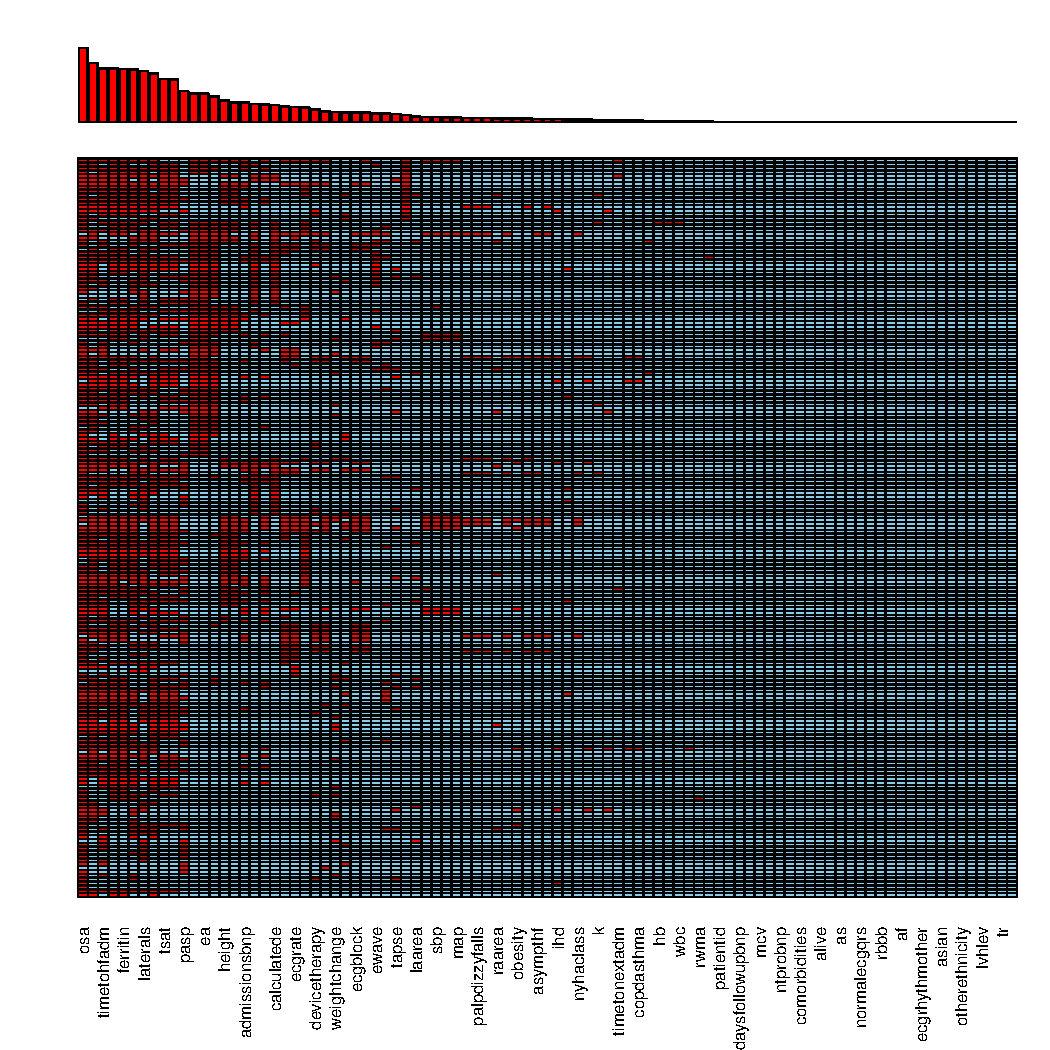
\includegraphics[width=1.1\textwidth]{doc/thesis/images/HFpEF_miss_dist.pdf}
    \caption[Missing values in HFpEF data set]{\textit{Missing values in HFpEF data set. Top:  the amount of missing values in each variable sorted in ascending order. Bottom: plot of the combinations of missing (red) and non-missing (blue) values in the HFpEF data set.}}
    \label{fig:HFpEF_missing}
\end{figure}

\newpage

\begin{figure}[h!]
    \centering
    \hspace*{-1cm}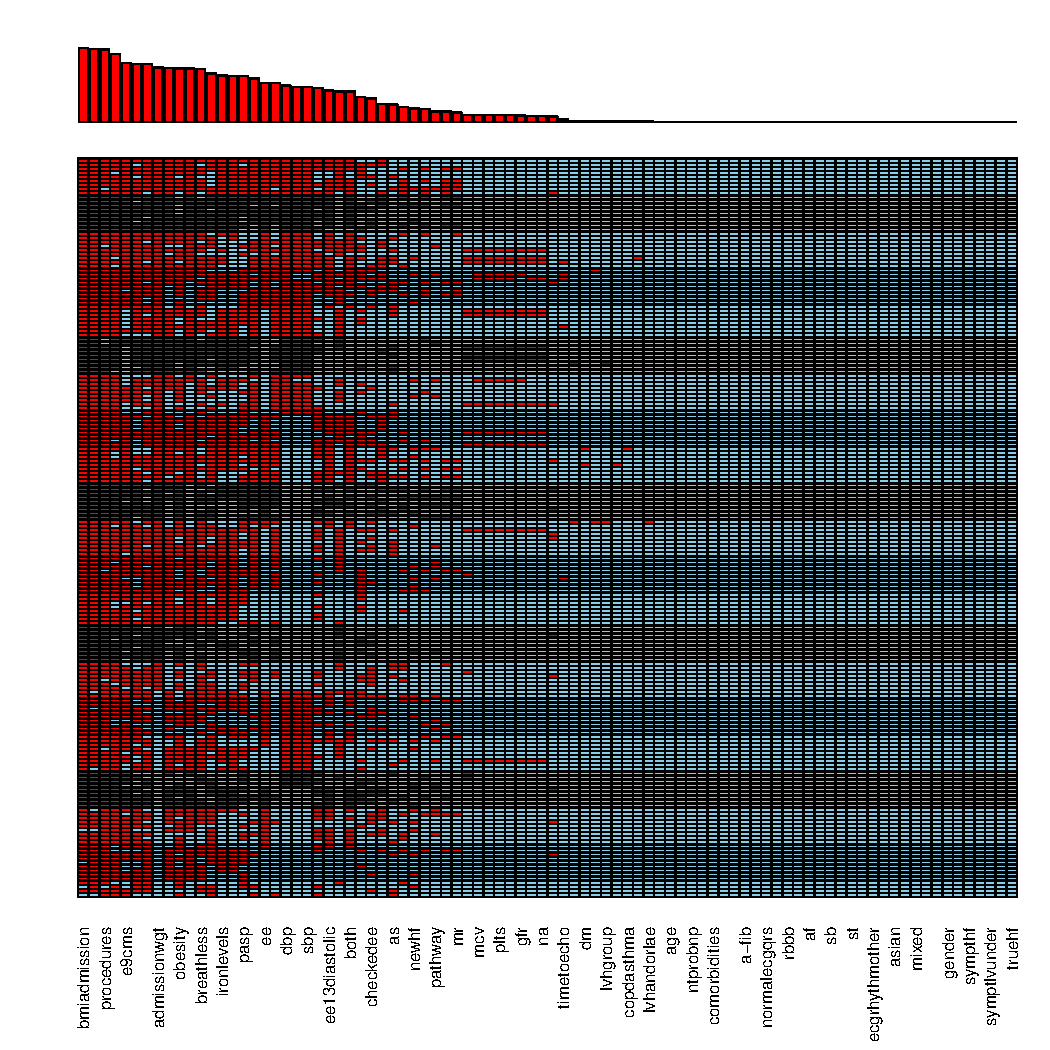
\includegraphics[width=1.1\textwidth]{doc/thesis/images/HFmrEF_miss_dist.pdf}
    \caption[Missing values in HFmrEF data set]{\textit{Missing values in HFmrEF data set. Top:  the amount of missing values in each variable sorted in ascending order. Bottom: plot of the combinations of missing (red) and non-missing (blue) values in the HFmrEF data set.}}
    \label{fig:HFmrEF_missing}
\end{figure}

\newpage

\begin{figure}[!ht]
\begin{subfigure}{\textwidth}
\centering
\resizebox{0.65\textwidth}{!}{\LARGE% Created by tikzDevice version 0.11 on 2018-05-09 15:09:57
% !TEX encoding = UTF-8 Unicode
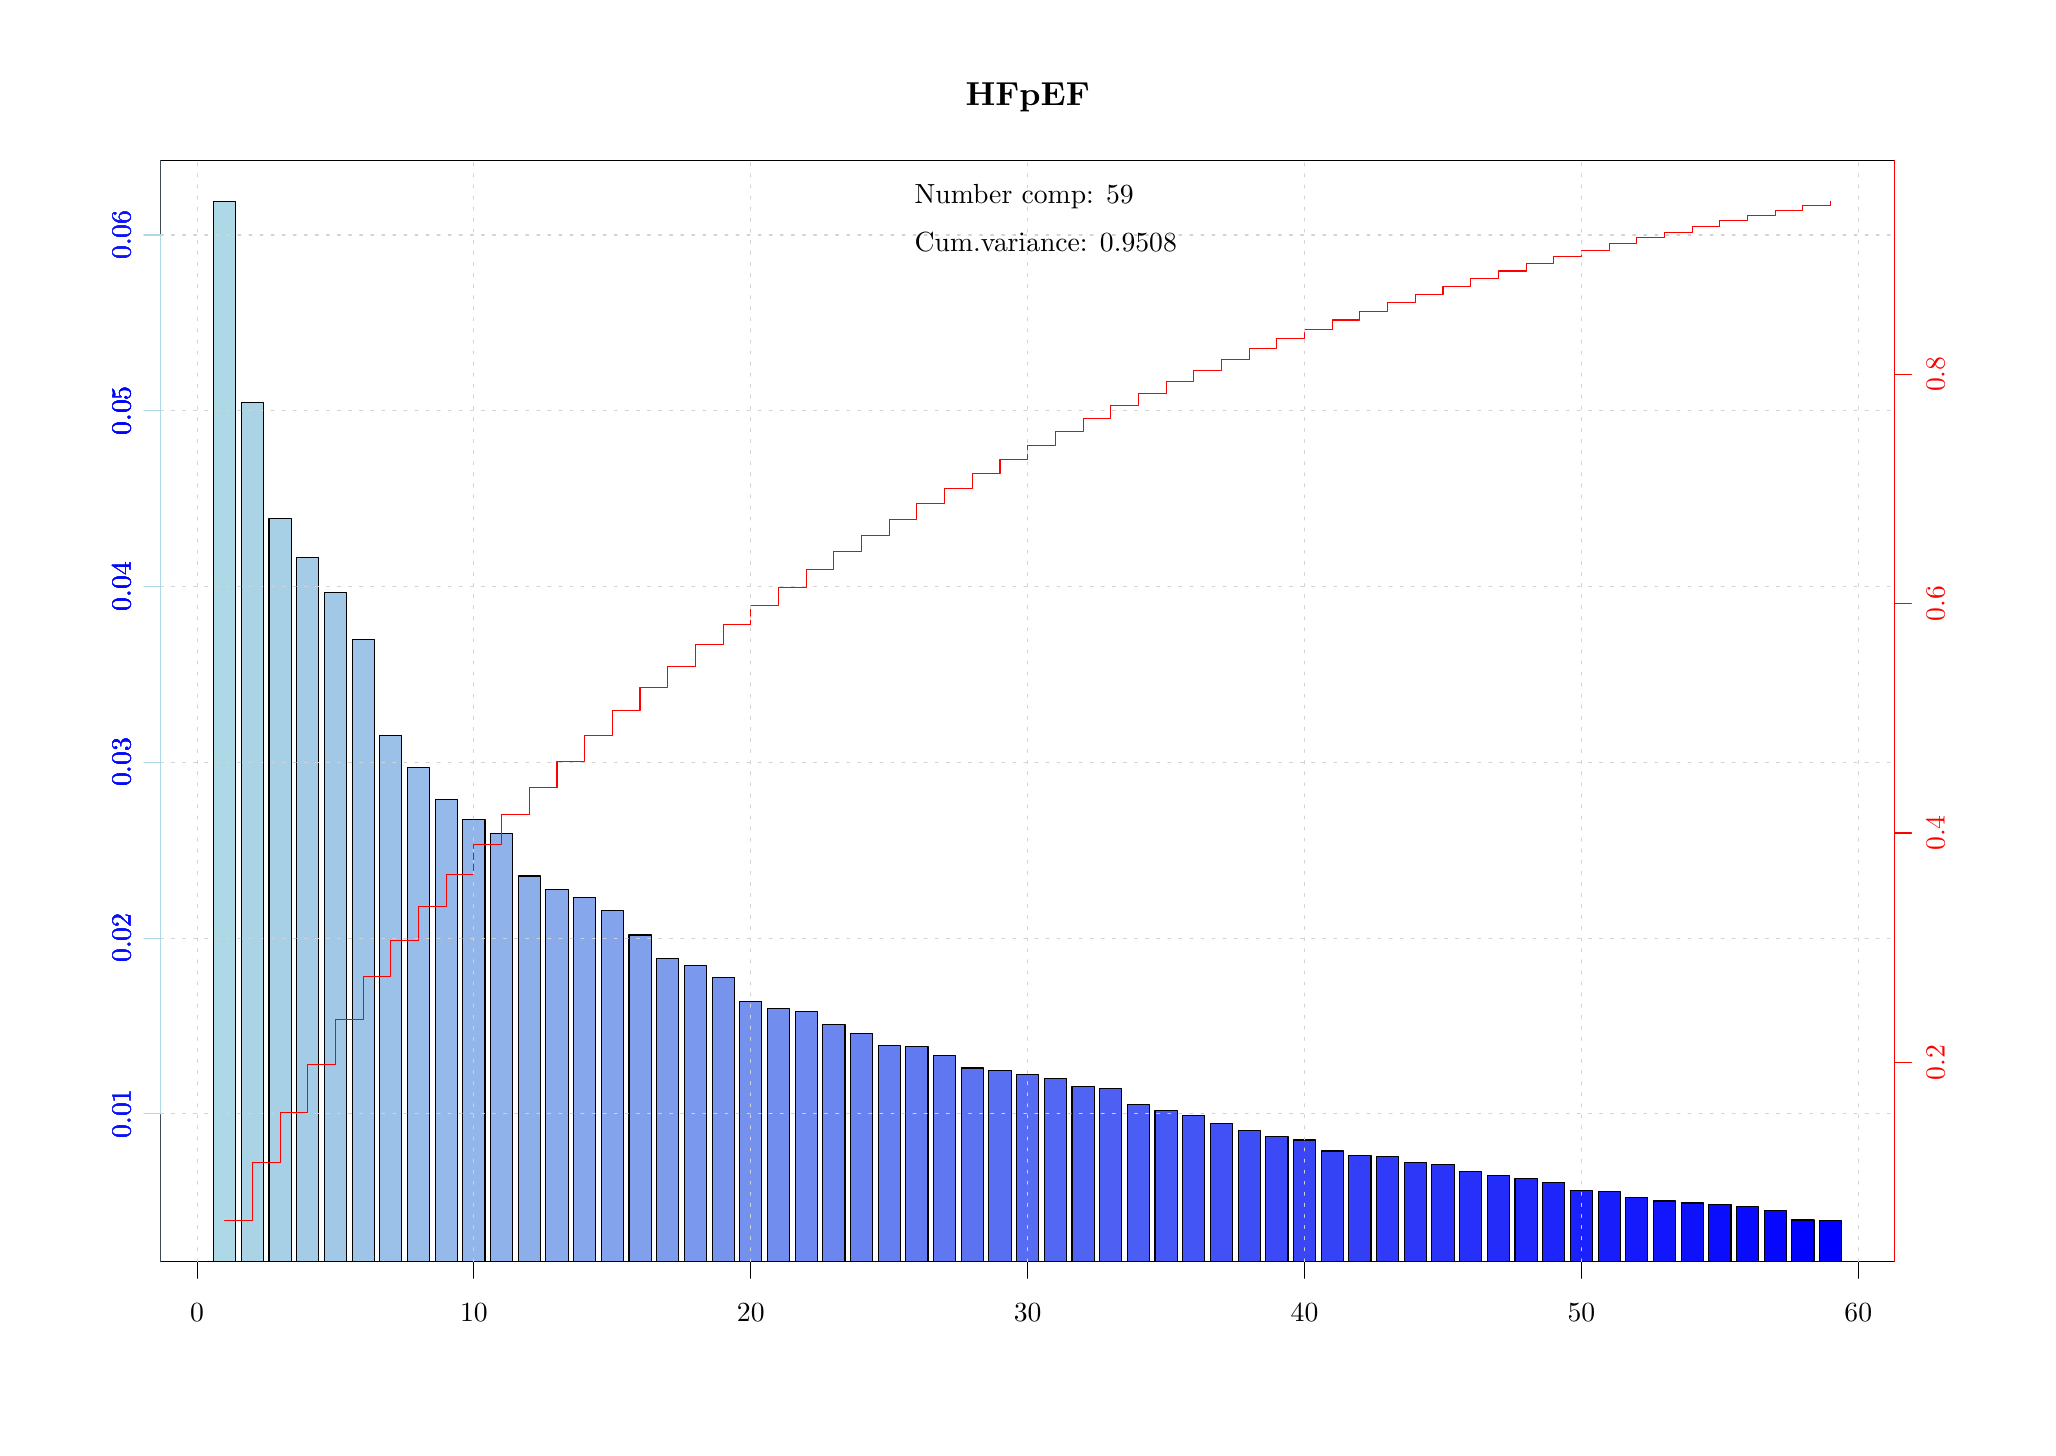
\begin{tikzpicture}[x=1pt,y=1pt]
\definecolor{fillColor}{RGB}{255,255,255}
\path[use as bounding box,fill=fillColor,fill opacity=0.00] (0,0) rectangle (722.70,505.89);
\begin{scope}
\path[clip] ( 48.00, 60.00) rectangle (674.70,457.89);
\definecolor{drawColor}{RGB}{0,0,0}
\definecolor{fillColor}{RGB}{173,216,230}

\path[draw=drawColor,line width= 0.4pt,line join=round,line cap=round,fill=fillColor] ( 67.21, 60.00) rectangle ( 75.21,443.15);
\definecolor{fillColor}{RGB}{170,212,230}

\path[draw=drawColor,line width= 0.4pt,line join=round,line cap=round,fill=fillColor] ( 77.21, 60.00) rectangle ( 85.22,370.44);
\definecolor{fillColor}{RGB}{167,208,230}

\path[draw=drawColor,line width= 0.4pt,line join=round,line cap=round,fill=fillColor] ( 87.22, 60.00) rectangle ( 95.22,328.47);
\definecolor{fillColor}{RGB}{164,204,231}

\path[draw=drawColor,line width= 0.4pt,line join=round,line cap=round,fill=fillColor] ( 97.22, 60.00) rectangle (105.23,314.38);
\definecolor{fillColor}{RGB}{161,201,231}

\path[draw=drawColor,line width= 0.4pt,line join=round,line cap=round,fill=fillColor] (107.23, 60.00) rectangle (115.23,301.74);
\definecolor{fillColor}{RGB}{158,197,232}

\path[draw=drawColor,line width= 0.4pt,line join=round,line cap=round,fill=fillColor] (117.23, 60.00) rectangle (125.24,284.82);
\definecolor{fillColor}{RGB}{155,193,232}

\path[draw=drawColor,line width= 0.4pt,line join=round,line cap=round,fill=fillColor] (127.24, 60.00) rectangle (135.24,250.18);
\definecolor{fillColor}{RGB}{152,189,233}

\path[draw=drawColor,line width= 0.4pt,line join=round,line cap=round,fill=fillColor] (137.24, 60.00) rectangle (145.25,238.52);
\definecolor{fillColor}{RGB}{149,186,233}

\path[draw=drawColor,line width= 0.4pt,line join=round,line cap=round,fill=fillColor] (147.25, 60.00) rectangle (155.25,226.92);
\definecolor{fillColor}{RGB}{146,182,233}

\path[draw=drawColor,line width= 0.4pt,line join=round,line cap=round,fill=fillColor] (157.25, 60.00) rectangle (165.26,219.61);
\definecolor{fillColor}{RGB}{143,178,234}

\path[draw=drawColor,line width= 0.4pt,line join=round,line cap=round,fill=fillColor] (167.26, 60.00) rectangle (175.26,214.78);
\definecolor{fillColor}{RGB}{140,175,234}

\path[draw=drawColor,line width= 0.4pt,line join=round,line cap=round,fill=fillColor] (177.26, 60.00) rectangle (185.27,199.34);
\definecolor{fillColor}{RGB}{137,171,235}

\path[draw=drawColor,line width= 0.4pt,line join=round,line cap=round,fill=fillColor] (187.27, 60.00) rectangle (195.27,194.32);
\definecolor{fillColor}{RGB}{134,167,235}

\path[draw=drawColor,line width= 0.4pt,line join=round,line cap=round,fill=fillColor] (197.27, 60.00) rectangle (205.28,191.69);
\definecolor{fillColor}{RGB}{131,163,236}

\path[draw=drawColor,line width= 0.4pt,line join=round,line cap=round,fill=fillColor] (207.28, 60.00) rectangle (215.28,186.94);
\definecolor{fillColor}{RGB}{128,160,236}

\path[draw=drawColor,line width= 0.4pt,line join=round,line cap=round,fill=fillColor] (217.28, 60.00) rectangle (225.28,178.03);
\definecolor{fillColor}{RGB}{125,156,236}

\path[draw=drawColor,line width= 0.4pt,line join=round,line cap=round,fill=fillColor] (227.29, 60.00) rectangle (235.29,169.60);
\definecolor{fillColor}{RGB}{122,152,237}

\path[draw=drawColor,line width= 0.4pt,line join=round,line cap=round,fill=fillColor] (237.29, 60.00) rectangle (245.29,166.92);
\definecolor{fillColor}{RGB}{119,148,237}

\path[draw=drawColor,line width= 0.4pt,line join=round,line cap=round,fill=fillColor] (247.30, 60.00) rectangle (255.30,162.63);
\definecolor{fillColor}{RGB}{116,145,238}

\path[draw=drawColor,line width= 0.4pt,line join=round,line cap=round,fill=fillColor] (257.30, 60.00) rectangle (265.30,154.09);
\definecolor{fillColor}{RGB}{113,141,238}

\path[draw=drawColor,line width= 0.4pt,line join=round,line cap=round,fill=fillColor] (267.30, 60.00) rectangle (275.31,151.41);
\definecolor{fillColor}{RGB}{110,137,239}

\path[draw=drawColor,line width= 0.4pt,line join=round,line cap=round,fill=fillColor] (277.31, 60.00) rectangle (285.31,150.50);
\definecolor{fillColor}{RGB}{107,134,239}

\path[draw=drawColor,line width= 0.4pt,line join=round,line cap=round,fill=fillColor] (287.31, 60.00) rectangle (295.32,145.67);
\definecolor{fillColor}{RGB}{104,130,239}

\path[draw=drawColor,line width= 0.4pt,line join=round,line cap=round,fill=fillColor] (297.32, 60.00) rectangle (305.32,142.52);
\definecolor{fillColor}{RGB}{101,126,240}

\path[draw=drawColor,line width= 0.4pt,line join=round,line cap=round,fill=fillColor] (307.32, 60.00) rectangle (315.33,138.07);
\definecolor{fillColor}{RGB}{98,122,240}

\path[draw=drawColor,line width= 0.4pt,line join=round,line cap=round,fill=fillColor] (317.33, 60.00) rectangle (325.33,137.58);
\definecolor{fillColor}{RGB}{95,119,241}

\path[draw=drawColor,line width= 0.4pt,line join=round,line cap=round,fill=fillColor] (327.33, 60.00) rectangle (335.34,134.45);
\definecolor{fillColor}{RGB}{92,115,241}

\path[draw=drawColor,line width= 0.4pt,line join=round,line cap=round,fill=fillColor] (337.34, 60.00) rectangle (345.34,129.97);
\definecolor{fillColor}{RGB}{89,111,242}

\path[draw=drawColor,line width= 0.4pt,line join=round,line cap=round,fill=fillColor] (347.34, 60.00) rectangle (355.35,128.91);
\definecolor{fillColor}{RGB}{86,108,242}

\path[draw=drawColor,line width= 0.4pt,line join=round,line cap=round,fill=fillColor] (357.35, 60.00) rectangle (365.35,127.68);
\definecolor{fillColor}{RGB}{83,104,242}

\path[draw=drawColor,line width= 0.4pt,line join=round,line cap=round,fill=fillColor] (367.35, 60.00) rectangle (375.36,126.21);
\definecolor{fillColor}{RGB}{80,100,243}

\path[draw=drawColor,line width= 0.4pt,line join=round,line cap=round,fill=fillColor] (377.36, 60.00) rectangle (385.36,123.34);
\definecolor{fillColor}{RGB}{77,96,243}

\path[draw=drawColor,line width= 0.4pt,line join=round,line cap=round,fill=fillColor] (387.36, 60.00) rectangle (395.37,122.47);
\definecolor{fillColor}{RGB}{74,93,244}

\path[draw=drawColor,line width= 0.4pt,line join=round,line cap=round,fill=fillColor] (397.37, 60.00) rectangle (405.37,116.77);
\definecolor{fillColor}{RGB}{71,89,244}

\path[draw=drawColor,line width= 0.4pt,line join=round,line cap=round,fill=fillColor] (407.37, 60.00) rectangle (415.38,114.47);
\definecolor{fillColor}{RGB}{68,85,245}

\path[draw=drawColor,line width= 0.4pt,line join=round,line cap=round,fill=fillColor] (417.38, 60.00) rectangle (425.38,112.87);
\definecolor{fillColor}{RGB}{65,81,245}

\path[draw=drawColor,line width= 0.4pt,line join=round,line cap=round,fill=fillColor] (427.38, 60.00) rectangle (435.39,109.91);
\definecolor{fillColor}{RGB}{62,78,245}

\path[draw=drawColor,line width= 0.4pt,line join=round,line cap=round,fill=fillColor] (437.39, 60.00) rectangle (445.39,107.53);
\definecolor{fillColor}{RGB}{59,74,246}

\path[draw=drawColor,line width= 0.4pt,line join=round,line cap=round,fill=fillColor] (447.39, 60.00) rectangle (455.40,105.12);
\definecolor{fillColor}{RGB}{56,70,246}

\path[draw=drawColor,line width= 0.4pt,line join=round,line cap=round,fill=fillColor] (457.40, 60.00) rectangle (465.40,103.94);
\definecolor{fillColor}{RGB}{53,67,247}

\path[draw=drawColor,line width= 0.4pt,line join=round,line cap=round,fill=fillColor] (467.40, 60.00) rectangle (475.40, 99.96);
\definecolor{fillColor}{RGB}{50,63,247}

\path[draw=drawColor,line width= 0.4pt,line join=round,line cap=round,fill=fillColor] (477.41, 60.00) rectangle (485.41, 98.48);
\definecolor{fillColor}{RGB}{47,59,248}

\path[draw=drawColor,line width= 0.4pt,line join=round,line cap=round,fill=fillColor] (487.41, 60.00) rectangle (495.41, 97.84);
\definecolor{fillColor}{RGB}{44,55,248}

\path[draw=drawColor,line width= 0.4pt,line join=round,line cap=round,fill=fillColor] (497.42, 60.00) rectangle (505.42, 95.79);
\definecolor{fillColor}{RGB}{41,52,248}

\path[draw=drawColor,line width= 0.4pt,line join=round,line cap=round,fill=fillColor] (507.42, 60.00) rectangle (515.42, 95.01);
\definecolor{fillColor}{RGB}{38,48,249}

\path[draw=drawColor,line width= 0.4pt,line join=round,line cap=round,fill=fillColor] (517.42, 60.00) rectangle (525.43, 92.41);
\definecolor{fillColor}{RGB}{35,44,249}

\path[draw=drawColor,line width= 0.4pt,line join=round,line cap=round,fill=fillColor] (527.43, 60.00) rectangle (535.43, 91.07);
\definecolor{fillColor}{RGB}{32,40,250}

\path[draw=drawColor,line width= 0.4pt,line join=round,line cap=round,fill=fillColor] (537.43, 60.00) rectangle (545.44, 89.97);
\definecolor{fillColor}{RGB}{29,37,250}

\path[draw=drawColor,line width= 0.4pt,line join=round,line cap=round,fill=fillColor] (547.44, 60.00) rectangle (555.44, 88.72);
\definecolor{fillColor}{RGB}{26,33,251}

\path[draw=drawColor,line width= 0.4pt,line join=round,line cap=round,fill=fillColor] (557.44, 60.00) rectangle (565.45, 85.69);
\definecolor{fillColor}{RGB}{23,29,251}

\path[draw=drawColor,line width= 0.4pt,line join=round,line cap=round,fill=fillColor] (567.45, 60.00) rectangle (575.45, 85.39);
\definecolor{fillColor}{RGB}{20,26,251}

\path[draw=drawColor,line width= 0.4pt,line join=round,line cap=round,fill=fillColor] (577.45, 60.00) rectangle (585.46, 83.21);
\definecolor{fillColor}{RGB}{17,22,252}

\path[draw=drawColor,line width= 0.4pt,line join=round,line cap=round,fill=fillColor] (587.46, 60.00) rectangle (595.46, 81.89);
\definecolor{fillColor}{RGB}{14,18,252}

\path[draw=drawColor,line width= 0.4pt,line join=round,line cap=round,fill=fillColor] (597.46, 60.00) rectangle (605.47, 81.17);
\definecolor{fillColor}{RGB}{11,14,253}

\path[draw=drawColor,line width= 0.4pt,line join=round,line cap=round,fill=fillColor] (607.47, 60.00) rectangle (615.47, 80.50);
\definecolor{fillColor}{RGB}{8,11,253}

\path[draw=drawColor,line width= 0.4pt,line join=round,line cap=round,fill=fillColor] (617.47, 60.00) rectangle (625.48, 79.78);
\definecolor{fillColor}{RGB}{5,7,254}

\path[draw=drawColor,line width= 0.4pt,line join=round,line cap=round,fill=fillColor] (627.48, 60.00) rectangle (635.48, 78.63);
\definecolor{fillColor}{RGB}{2,3,254}

\path[draw=drawColor,line width= 0.4pt,line join=round,line cap=round,fill=fillColor] (637.48, 60.00) rectangle (645.49, 75.04);
\definecolor{fillColor}{RGB}{0,0,255}

\path[draw=drawColor,line width= 0.4pt,line join=round,line cap=round,fill=fillColor] (647.49, 60.00) rectangle (655.49, 74.74);
\end{scope}
\begin{scope}
\path[clip] (  0.00,  0.00) rectangle (722.70,505.89);
\definecolor{drawColor}{RGB}{0,0,0}

\node[text=drawColor,anchor=base,inner sep=0pt, outer sep=0pt, scale=  1.20] at (361.35,477.75) {\bfseries HFpEF};
\end{scope}
\begin{scope}
\path[clip] (  0.00,  0.00) rectangle (722.70,505.89);
\definecolor{drawColor}{RGB}{0,0,0}

\path[draw=drawColor,line width= 0.4pt,line join=round,line cap=round] ( 48.00, 60.00) --
	(674.70, 60.00) --
	(674.70,457.89) --
	( 48.00,457.89) --
	( 48.00, 60.00);

\path[draw=drawColor,line width= 0.4pt,line join=round,line cap=round] ( 61.21, 60.00) -- (661.49, 60.00);

\path[draw=drawColor,line width= 0.4pt,line join=round,line cap=round] ( 61.21, 60.00) -- ( 61.21, 54.00);

\path[draw=drawColor,line width= 0.4pt,line join=round,line cap=round] (161.25, 60.00) -- (161.25, 54.00);

\path[draw=drawColor,line width= 0.4pt,line join=round,line cap=round] (261.30, 60.00) -- (261.30, 54.00);

\path[draw=drawColor,line width= 0.4pt,line join=round,line cap=round] (361.35, 60.00) -- (361.35, 54.00);

\path[draw=drawColor,line width= 0.4pt,line join=round,line cap=round] (461.40, 60.00) -- (461.40, 54.00);

\path[draw=drawColor,line width= 0.4pt,line join=round,line cap=round] (561.45, 60.00) -- (561.45, 54.00);

\path[draw=drawColor,line width= 0.4pt,line join=round,line cap=round] (661.49, 60.00) -- (661.49, 54.00);

\node[text=drawColor,anchor=base,inner sep=0pt, outer sep=0pt, scale=  1.00] at ( 61.21, 38.40) {0};

\node[text=drawColor,anchor=base,inner sep=0pt, outer sep=0pt, scale=  1.00] at (161.25, 38.40) {10};

\node[text=drawColor,anchor=base,inner sep=0pt, outer sep=0pt, scale=  1.00] at (261.30, 38.40) {20};

\node[text=drawColor,anchor=base,inner sep=0pt, outer sep=0pt, scale=  1.00] at (361.35, 38.40) {30};

\node[text=drawColor,anchor=base,inner sep=0pt, outer sep=0pt, scale=  1.00] at (461.40, 38.40) {40};

\node[text=drawColor,anchor=base,inner sep=0pt, outer sep=0pt, scale=  1.00] at (561.45, 38.40) {50};

\node[text=drawColor,anchor=base,inner sep=0pt, outer sep=0pt, scale=  1.00] at (661.49, 38.40) {60};
\definecolor{drawColor}{RGB}{173,216,230}

\path[draw=drawColor,line width= 0.4pt,line join=round,line cap=round] ( 48.00,113.39) -- ( 48.00,430.96);

\path[draw=drawColor,line width= 0.4pt,line join=round,line cap=round] ( 48.00,113.39) -- ( 42.00,113.39);

\path[draw=drawColor,line width= 0.4pt,line join=round,line cap=round] ( 48.00,176.90) -- ( 42.00,176.90);

\path[draw=drawColor,line width= 0.4pt,line join=round,line cap=round] ( 48.00,240.42) -- ( 42.00,240.42);

\path[draw=drawColor,line width= 0.4pt,line join=round,line cap=round] ( 48.00,303.93) -- ( 42.00,303.93);

\path[draw=drawColor,line width= 0.4pt,line join=round,line cap=round] ( 48.00,367.44) -- ( 42.00,367.44);

\path[draw=drawColor,line width= 0.4pt,line join=round,line cap=round] ( 48.00,430.96) -- ( 42.00,430.96);

\node[text=drawColor,rotate= 90.00,anchor=base,inner sep=0pt, outer sep=0pt, scale=  1.00] at ( 37.20,113.39) {0.01};
\definecolor{drawColor}{RGB}{170,212,230}

\node[text=drawColor,rotate= 90.00,anchor=base,inner sep=0pt, outer sep=0pt, scale=  1.00] at ( 37.20,176.90) {0.02};
\definecolor{drawColor}{RGB}{167,208,230}

\node[text=drawColor,rotate= 90.00,anchor=base,inner sep=0pt, outer sep=0pt, scale=  1.00] at ( 37.20,240.42) {0.03};
\definecolor{drawColor}{RGB}{164,204,231}

\node[text=drawColor,rotate= 90.00,anchor=base,inner sep=0pt, outer sep=0pt, scale=  1.00] at ( 37.20,303.93) {0.04};
\definecolor{drawColor}{RGB}{161,201,231}

\node[text=drawColor,rotate= 90.00,anchor=base,inner sep=0pt, outer sep=0pt, scale=  1.00] at ( 37.20,367.44) {0.05};
\definecolor{drawColor}{RGB}{158,197,232}

\node[text=drawColor,rotate= 90.00,anchor=base,inner sep=0pt, outer sep=0pt, scale=  1.00] at ( 37.20,430.96) {0.06};
\definecolor{drawColor}{RGB}{155,193,232}

\node[text=drawColor,rotate= 90.00,anchor=base,inner sep=0pt, outer sep=0pt, scale=  1.00] at ( 37.20,113.39) {0.01};
\definecolor{drawColor}{RGB}{152,189,233}

\node[text=drawColor,rotate= 90.00,anchor=base,inner sep=0pt, outer sep=0pt, scale=  1.00] at ( 37.20,176.90) {0.02};
\definecolor{drawColor}{RGB}{149,186,233}

\node[text=drawColor,rotate= 90.00,anchor=base,inner sep=0pt, outer sep=0pt, scale=  1.00] at ( 37.20,240.42) {0.03};
\definecolor{drawColor}{RGB}{146,182,233}

\node[text=drawColor,rotate= 90.00,anchor=base,inner sep=0pt, outer sep=0pt, scale=  1.00] at ( 37.20,303.93) {0.04};
\definecolor{drawColor}{RGB}{143,178,234}

\node[text=drawColor,rotate= 90.00,anchor=base,inner sep=0pt, outer sep=0pt, scale=  1.00] at ( 37.20,367.44) {0.05};
\definecolor{drawColor}{RGB}{140,175,234}

\node[text=drawColor,rotate= 90.00,anchor=base,inner sep=0pt, outer sep=0pt, scale=  1.00] at ( 37.20,430.96) {0.06};
\definecolor{drawColor}{RGB}{137,171,235}

\node[text=drawColor,rotate= 90.00,anchor=base,inner sep=0pt, outer sep=0pt, scale=  1.00] at ( 37.20,113.39) {0.01};
\definecolor{drawColor}{RGB}{134,167,235}

\node[text=drawColor,rotate= 90.00,anchor=base,inner sep=0pt, outer sep=0pt, scale=  1.00] at ( 37.20,176.90) {0.02};
\definecolor{drawColor}{RGB}{131,163,236}

\node[text=drawColor,rotate= 90.00,anchor=base,inner sep=0pt, outer sep=0pt, scale=  1.00] at ( 37.20,240.42) {0.03};
\definecolor{drawColor}{RGB}{128,160,236}

\node[text=drawColor,rotate= 90.00,anchor=base,inner sep=0pt, outer sep=0pt, scale=  1.00] at ( 37.20,303.93) {0.04};
\definecolor{drawColor}{RGB}{125,156,236}

\node[text=drawColor,rotate= 90.00,anchor=base,inner sep=0pt, outer sep=0pt, scale=  1.00] at ( 37.20,367.44) {0.05};
\definecolor{drawColor}{RGB}{122,152,237}

\node[text=drawColor,rotate= 90.00,anchor=base,inner sep=0pt, outer sep=0pt, scale=  1.00] at ( 37.20,430.96) {0.06};
\definecolor{drawColor}{RGB}{119,148,237}

\node[text=drawColor,rotate= 90.00,anchor=base,inner sep=0pt, outer sep=0pt, scale=  1.00] at ( 37.20,113.39) {0.01};
\definecolor{drawColor}{RGB}{116,145,238}

\node[text=drawColor,rotate= 90.00,anchor=base,inner sep=0pt, outer sep=0pt, scale=  1.00] at ( 37.20,176.90) {0.02};
\definecolor{drawColor}{RGB}{113,141,238}

\node[text=drawColor,rotate= 90.00,anchor=base,inner sep=0pt, outer sep=0pt, scale=  1.00] at ( 37.20,240.42) {0.03};
\definecolor{drawColor}{RGB}{110,137,239}

\node[text=drawColor,rotate= 90.00,anchor=base,inner sep=0pt, outer sep=0pt, scale=  1.00] at ( 37.20,303.93) {0.04};
\definecolor{drawColor}{RGB}{107,134,239}

\node[text=drawColor,rotate= 90.00,anchor=base,inner sep=0pt, outer sep=0pt, scale=  1.00] at ( 37.20,367.44) {0.05};
\definecolor{drawColor}{RGB}{104,130,239}

\node[text=drawColor,rotate= 90.00,anchor=base,inner sep=0pt, outer sep=0pt, scale=  1.00] at ( 37.20,430.96) {0.06};
\definecolor{drawColor}{RGB}{101,126,240}

\node[text=drawColor,rotate= 90.00,anchor=base,inner sep=0pt, outer sep=0pt, scale=  1.00] at ( 37.20,113.39) {0.01};
\definecolor{drawColor}{RGB}{98,122,240}

\node[text=drawColor,rotate= 90.00,anchor=base,inner sep=0pt, outer sep=0pt, scale=  1.00] at ( 37.20,176.90) {0.02};
\definecolor{drawColor}{RGB}{95,119,241}

\node[text=drawColor,rotate= 90.00,anchor=base,inner sep=0pt, outer sep=0pt, scale=  1.00] at ( 37.20,240.42) {0.03};
\definecolor{drawColor}{RGB}{92,115,241}

\node[text=drawColor,rotate= 90.00,anchor=base,inner sep=0pt, outer sep=0pt, scale=  1.00] at ( 37.20,303.93) {0.04};
\definecolor{drawColor}{RGB}{89,111,242}

\node[text=drawColor,rotate= 90.00,anchor=base,inner sep=0pt, outer sep=0pt, scale=  1.00] at ( 37.20,367.44) {0.05};
\definecolor{drawColor}{RGB}{86,108,242}

\node[text=drawColor,rotate= 90.00,anchor=base,inner sep=0pt, outer sep=0pt, scale=  1.00] at ( 37.20,430.96) {0.06};
\definecolor{drawColor}{RGB}{83,104,242}

\node[text=drawColor,rotate= 90.00,anchor=base,inner sep=0pt, outer sep=0pt, scale=  1.00] at ( 37.20,113.39) {0.01};
\definecolor{drawColor}{RGB}{80,100,243}

\node[text=drawColor,rotate= 90.00,anchor=base,inner sep=0pt, outer sep=0pt, scale=  1.00] at ( 37.20,176.90) {0.02};
\definecolor{drawColor}{RGB}{77,96,243}

\node[text=drawColor,rotate= 90.00,anchor=base,inner sep=0pt, outer sep=0pt, scale=  1.00] at ( 37.20,240.42) {0.03};
\definecolor{drawColor}{RGB}{74,93,244}

\node[text=drawColor,rotate= 90.00,anchor=base,inner sep=0pt, outer sep=0pt, scale=  1.00] at ( 37.20,303.93) {0.04};
\definecolor{drawColor}{RGB}{71,89,244}

\node[text=drawColor,rotate= 90.00,anchor=base,inner sep=0pt, outer sep=0pt, scale=  1.00] at ( 37.20,367.44) {0.05};
\definecolor{drawColor}{RGB}{68,85,245}

\node[text=drawColor,rotate= 90.00,anchor=base,inner sep=0pt, outer sep=0pt, scale=  1.00] at ( 37.20,430.96) {0.06};
\definecolor{drawColor}{RGB}{65,81,245}

\node[text=drawColor,rotate= 90.00,anchor=base,inner sep=0pt, outer sep=0pt, scale=  1.00] at ( 37.20,113.39) {0.01};
\definecolor{drawColor}{RGB}{62,78,245}

\node[text=drawColor,rotate= 90.00,anchor=base,inner sep=0pt, outer sep=0pt, scale=  1.00] at ( 37.20,176.90) {0.02};
\definecolor{drawColor}{RGB}{59,74,246}

\node[text=drawColor,rotate= 90.00,anchor=base,inner sep=0pt, outer sep=0pt, scale=  1.00] at ( 37.20,240.42) {0.03};
\definecolor{drawColor}{RGB}{56,70,246}

\node[text=drawColor,rotate= 90.00,anchor=base,inner sep=0pt, outer sep=0pt, scale=  1.00] at ( 37.20,303.93) {0.04};
\definecolor{drawColor}{RGB}{53,67,247}

\node[text=drawColor,rotate= 90.00,anchor=base,inner sep=0pt, outer sep=0pt, scale=  1.00] at ( 37.20,367.44) {0.05};
\definecolor{drawColor}{RGB}{50,63,247}

\node[text=drawColor,rotate= 90.00,anchor=base,inner sep=0pt, outer sep=0pt, scale=  1.00] at ( 37.20,430.96) {0.06};
\definecolor{drawColor}{RGB}{47,59,248}

\node[text=drawColor,rotate= 90.00,anchor=base,inner sep=0pt, outer sep=0pt, scale=  1.00] at ( 37.20,113.39) {0.01};
\definecolor{drawColor}{RGB}{44,55,248}

\node[text=drawColor,rotate= 90.00,anchor=base,inner sep=0pt, outer sep=0pt, scale=  1.00] at ( 37.20,176.90) {0.02};
\definecolor{drawColor}{RGB}{41,52,248}

\node[text=drawColor,rotate= 90.00,anchor=base,inner sep=0pt, outer sep=0pt, scale=  1.00] at ( 37.20,240.42) {0.03};
\definecolor{drawColor}{RGB}{38,48,249}

\node[text=drawColor,rotate= 90.00,anchor=base,inner sep=0pt, outer sep=0pt, scale=  1.00] at ( 37.20,303.93) {0.04};
\definecolor{drawColor}{RGB}{35,44,249}

\node[text=drawColor,rotate= 90.00,anchor=base,inner sep=0pt, outer sep=0pt, scale=  1.00] at ( 37.20,367.44) {0.05};
\definecolor{drawColor}{RGB}{32,40,250}

\node[text=drawColor,rotate= 90.00,anchor=base,inner sep=0pt, outer sep=0pt, scale=  1.00] at ( 37.20,430.96) {0.06};
\definecolor{drawColor}{RGB}{29,37,250}

\node[text=drawColor,rotate= 90.00,anchor=base,inner sep=0pt, outer sep=0pt, scale=  1.00] at ( 37.20,113.39) {0.01};
\definecolor{drawColor}{RGB}{26,33,251}

\node[text=drawColor,rotate= 90.00,anchor=base,inner sep=0pt, outer sep=0pt, scale=  1.00] at ( 37.20,176.90) {0.02};
\definecolor{drawColor}{RGB}{23,29,251}

\node[text=drawColor,rotate= 90.00,anchor=base,inner sep=0pt, outer sep=0pt, scale=  1.00] at ( 37.20,240.42) {0.03};
\definecolor{drawColor}{RGB}{20,26,251}

\node[text=drawColor,rotate= 90.00,anchor=base,inner sep=0pt, outer sep=0pt, scale=  1.00] at ( 37.20,303.93) {0.04};
\definecolor{drawColor}{RGB}{17,22,252}

\node[text=drawColor,rotate= 90.00,anchor=base,inner sep=0pt, outer sep=0pt, scale=  1.00] at ( 37.20,367.44) {0.05};
\definecolor{drawColor}{RGB}{14,18,252}

\node[text=drawColor,rotate= 90.00,anchor=base,inner sep=0pt, outer sep=0pt, scale=  1.00] at ( 37.20,430.96) {0.06};
\definecolor{drawColor}{RGB}{11,14,253}

\node[text=drawColor,rotate= 90.00,anchor=base,inner sep=0pt, outer sep=0pt, scale=  1.00] at ( 37.20,113.39) {0.01};
\definecolor{drawColor}{RGB}{8,11,253}

\node[text=drawColor,rotate= 90.00,anchor=base,inner sep=0pt, outer sep=0pt, scale=  1.00] at ( 37.20,176.90) {0.02};
\definecolor{drawColor}{RGB}{5,7,254}

\node[text=drawColor,rotate= 90.00,anchor=base,inner sep=0pt, outer sep=0pt, scale=  1.00] at ( 37.20,240.42) {0.03};
\definecolor{drawColor}{RGB}{2,3,254}

\node[text=drawColor,rotate= 90.00,anchor=base,inner sep=0pt, outer sep=0pt, scale=  1.00] at ( 37.20,303.93) {0.04};
\definecolor{drawColor}{RGB}{0,0,255}

\node[text=drawColor,rotate= 90.00,anchor=base,inner sep=0pt, outer sep=0pt, scale=  1.00] at ( 37.20,367.44) {0.05};
\end{scope}
\begin{scope}
\path[clip] ( 48.00, 60.00) rectangle (674.70,457.89);
\definecolor{drawColor}{RGB}{173,216,230}

\path[draw=drawColor,line width= 0.4pt,line join=round,line cap=round] ( 48.00, 60.00) -- ( 48.00,457.89);
\definecolor{drawColor}{RGB}{255,0,0}

\path[draw=drawColor,line width= 0.4pt,line join=round,line cap=round] ( 71.21, 74.74) --
	( 81.22, 74.74) --
	( 81.22, 95.66) --
	( 91.22, 95.66) --
	( 91.22,113.84) --
	(101.23,113.84) --
	(101.23,131.10) --
	(111.23,131.10) --
	(111.23,147.54) --
	(121.24,147.54) --
	(121.24,162.87) --
	(131.24,162.87) --
	(131.24,175.94) --
	(141.24,175.94) --
	(141.24,188.25) --
	(151.25,188.25) --
	(151.25,199.81) --
	(161.25,199.81) --
	(161.25,210.88) --
	(171.26,210.88) --
	(171.26,221.64) --
	(181.26,221.64) --
	(181.26,231.40) --
	(191.27,231.40) --
	(191.27,240.82) --
	(201.27,240.82) --
	(201.27,250.08) --
	(211.28,250.08) --
	(211.28,259.02) --
	(221.28,259.02) --
	(221.28,267.39) --
	(231.29,267.39) --
	(231.29,275.20) --
	(241.29,275.20) --
	(241.29,282.84) --
	(251.30,282.84) --
	(251.30,290.20) --
	(261.30,290.20) --
	(261.30,297.00) --
	(271.31,297.00) --
	(271.31,303.62) --
	(281.31,303.62) --
	(281.31,310.19) --
	(291.32,310.19) --
	(291.32,316.44) --
	(301.32,316.44) --
	(301.32,322.49) --
	(311.33,322.49) --
	(311.33,328.24) --
	(321.33,328.24) --
	(321.33,333.97) --
	(331.34,333.97) --
	(331.34,339.49) --
	(341.34,339.49) --
	(341.34,344.71) --
	(351.35,344.71) --
	(351.35,349.87) --
	(361.35,349.87) --
	(361.35,354.95) --
	(371.35,354.95) --
	(371.35,359.93) --
	(381.36,359.93) --
	(381.36,364.73) --
	(391.36,364.73) --
	(391.36,369.46) --
	(401.37,369.46) --
	(401.37,373.83) --
	(411.37,373.83) --
	(411.37,378.05) --
	(421.38,378.05) --
	(421.38,382.16) --
	(431.38,382.16) --
	(431.38,386.07) --
	(441.39,386.07) --
	(441.39,389.84) --
	(451.39,389.84) --
	(451.39,393.44) --
	(461.40,393.44) --
	(461.40,396.97) --
	(471.40,396.97) --
	(471.40,400.24) --
	(481.41,400.24) --
	(481.41,403.41) --
	(491.41,403.41) --
	(491.41,406.54) --
	(501.42,406.54) --
	(501.42,409.54) --
	(511.42,409.54) --
	(511.42,412.48) --
	(521.43,412.48) --
	(521.43,415.26) --
	(531.43,415.26) --
	(531.43,417.95) --
	(541.44,417.95) --
	(541.44,420.56) --
	(551.44,420.56) --
	(551.44,423.10) --
	(561.45,423.10) --
	(561.45,425.44) --
	(571.45,425.44) --
	(571.45,427.75) --
	(581.46,427.75) --
	(581.46,429.93) --
	(591.46,429.93) --
	(591.46,432.02) --
	(601.46,432.02) --
	(601.46,434.06) --
	(611.47,434.06) --
	(611.47,436.06) --
	(621.47,436.06) --
	(621.47,438.01) --
	(631.48,438.01) --
	(631.48,439.89) --
	(641.48,439.89) --
	(641.48,441.53) --
	(651.49,441.53) --
	(651.49,443.15);
\end{scope}
\begin{scope}
\path[clip] (  0.00,  0.00) rectangle (722.70,505.89);
\definecolor{drawColor}{RGB}{255,0,0}

\path[draw=drawColor,line width= 0.4pt,line join=round,line cap=round] (674.70,131.97) -- (674.70,380.66);

\path[draw=drawColor,line width= 0.4pt,line join=round,line cap=round] (674.70,131.97) -- (680.70,131.97);

\path[draw=drawColor,line width= 0.4pt,line join=round,line cap=round] (674.70,214.87) -- (680.70,214.87);

\path[draw=drawColor,line width= 0.4pt,line join=round,line cap=round] (674.70,297.77) -- (680.70,297.77);

\path[draw=drawColor,line width= 0.4pt,line join=round,line cap=round] (674.70,380.66) -- (680.70,380.66);

\node[text=drawColor,rotate= 90.00,anchor=base,inner sep=0pt, outer sep=0pt, scale=  1.00] at (692.70,131.97) {0.2};

\node[text=drawColor,rotate= 90.00,anchor=base,inner sep=0pt, outer sep=0pt, scale=  1.00] at (692.70,214.87) {0.4};

\node[text=drawColor,rotate= 90.00,anchor=base,inner sep=0pt, outer sep=0pt, scale=  1.00] at (692.70,297.77) {0.6};

\node[text=drawColor,rotate= 90.00,anchor=base,inner sep=0pt, outer sep=0pt, scale=  1.00] at (692.70,380.66) {0.8};
\end{scope}
\begin{scope}
\path[clip] ( 48.00, 60.00) rectangle (674.70,457.89);
\definecolor{drawColor}{RGB}{255,0,0}

\path[draw=drawColor,line width= 0.4pt,line join=round,line cap=round] (674.70, 60.00) -- (674.70,457.89);
\definecolor{drawColor}{RGB}{211,211,211}

\path[draw=drawColor,line width= 0.4pt,dash pattern=on 1pt off 3pt ,line join=round,line cap=round] ( 61.21, 60.00) -- ( 61.21,457.89);

\path[draw=drawColor,line width= 0.4pt,dash pattern=on 1pt off 3pt ,line join=round,line cap=round] (161.25, 60.00) -- (161.25,457.89);

\path[draw=drawColor,line width= 0.4pt,dash pattern=on 1pt off 3pt ,line join=round,line cap=round] (261.30, 60.00) -- (261.30,457.89);

\path[draw=drawColor,line width= 0.4pt,dash pattern=on 1pt off 3pt ,line join=round,line cap=round] (361.35, 60.00) -- (361.35,457.89);

\path[draw=drawColor,line width= 0.4pt,dash pattern=on 1pt off 3pt ,line join=round,line cap=round] (461.40, 60.00) -- (461.40,457.89);

\path[draw=drawColor,line width= 0.4pt,dash pattern=on 1pt off 3pt ,line join=round,line cap=round] (561.45, 60.00) -- (561.45,457.89);

\path[draw=drawColor,line width= 0.4pt,dash pattern=on 1pt off 3pt ,line join=round,line cap=round] (661.49, 60.00) -- (661.49,457.89);

\path[draw=drawColor,line width= 0.4pt,dash pattern=on 1pt off 3pt ,line join=round,line cap=round] ( 48.00,113.39) -- (674.70,113.39);

\path[draw=drawColor,line width= 0.4pt,dash pattern=on 1pt off 3pt ,line join=round,line cap=round] ( 48.00,176.90) -- (674.70,176.90);

\path[draw=drawColor,line width= 0.4pt,dash pattern=on 1pt off 3pt ,line join=round,line cap=round] ( 48.00,240.42) -- (674.70,240.42);

\path[draw=drawColor,line width= 0.4pt,dash pattern=on 1pt off 3pt ,line join=round,line cap=round] ( 48.00,303.93) -- (674.70,303.93);

\path[draw=drawColor,line width= 0.4pt,dash pattern=on 1pt off 3pt ,line join=round,line cap=round] ( 48.00,367.44) -- (674.70,367.44);

\path[draw=drawColor,line width= 0.4pt,dash pattern=on 1pt off 3pt ,line join=round,line cap=round] ( 48.00,430.96) -- (674.70,430.96);
\definecolor{drawColor}{RGB}{0,0,0}

\node[text=drawColor,anchor=base west,inner sep=0pt, outer sep=0pt, scale=  1.00] at (320.51,442.37) {Number comp: 59};

\node[text=drawColor,anchor=base west,inner sep=0pt, outer sep=0pt, scale=  1.00] at (320.51,425) {Cum.variance: 0.9508};
\end{scope}
\end{tikzpicture}
}
\caption{\textit{Explained variance (blue) and cumulative explained variance (red) for $n = 59$ principal components in HFpEF data set.}}
\end{subfigure}
\begin{subfigure}{\textwidth}
\centering
\resizebox{0.65\textwidth}{!}{\LARGE% Created by tikzDevice version 0.11 on 2018-05-09 14:27:11
% !TEX encoding = UTF-8 Unicode
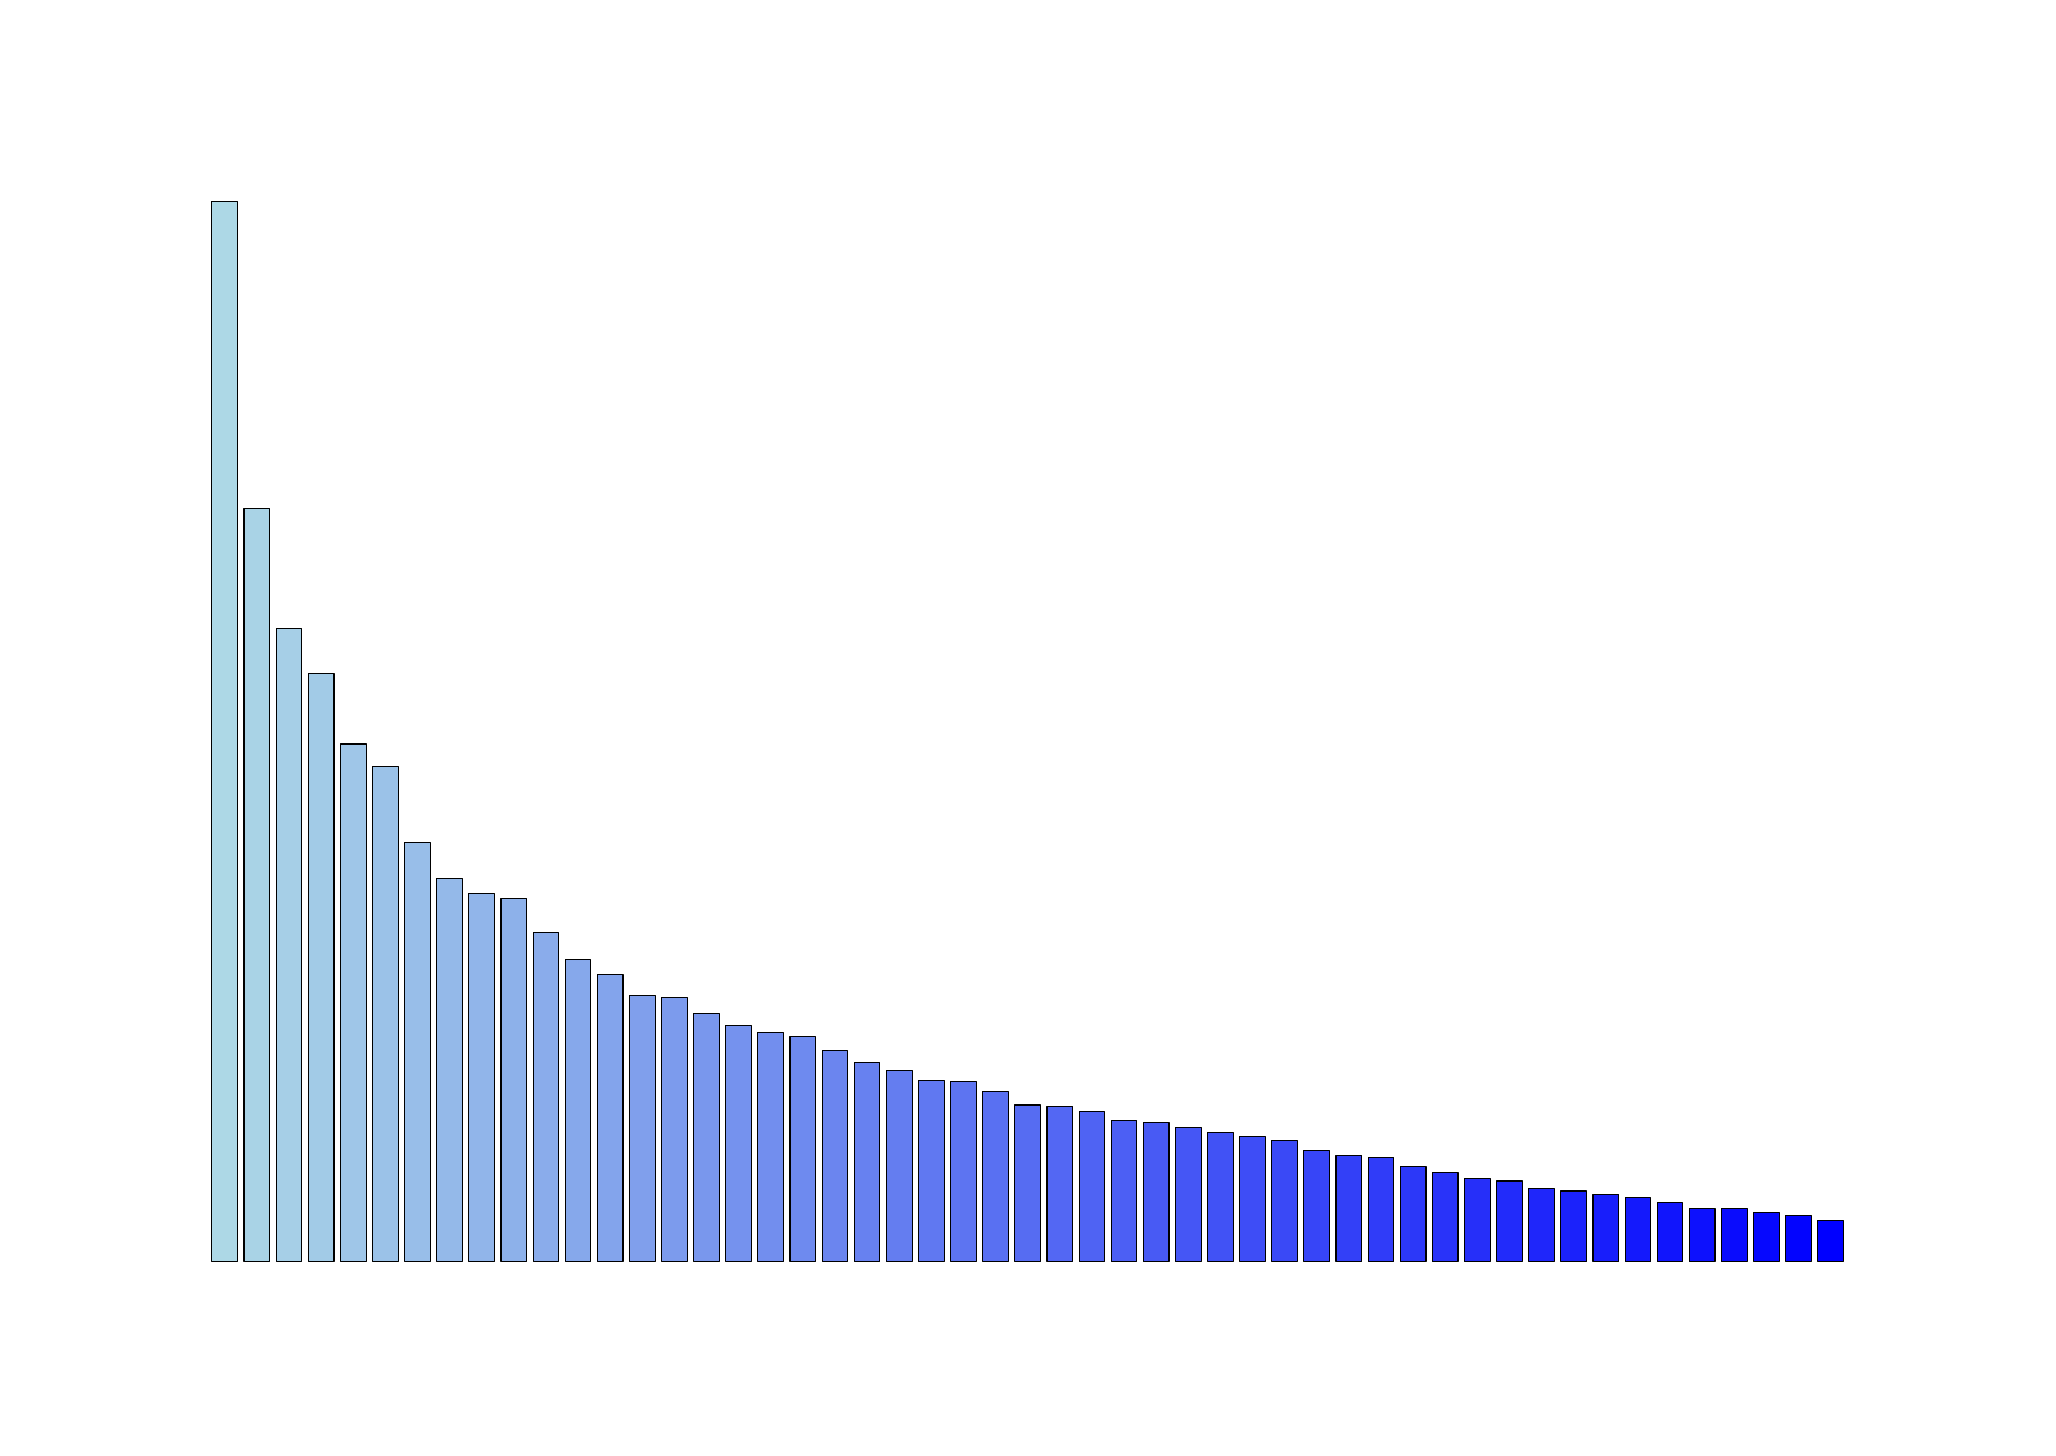
\begin{tikzpicture}[x=1pt,y=1pt]
\definecolor{fillColor}{RGB}{255,255,255}
\path[use as bounding box,fill=fillColor,fill opacity=0.00] (0,0) rectangle (722.70,505.89);
\begin{scope}
\path[clip] ( 48.00, 60.00) rectangle (674.70,457.89);
\definecolor{drawColor}{RGB}{0,0,0}
\definecolor{fillColor}{RGB}{173,216,230}

\path[draw=drawColor,line width= 0.4pt,line join=round,line cap=round,fill=fillColor] ( 66.57, 60.00) rectangle ( 75.85,443.15);
\definecolor{fillColor}{RGB}{169,211,230}

\path[draw=drawColor,line width= 0.4pt,line join=round,line cap=round,fill=fillColor] ( 78.17, 60.00) rectangle ( 87.46,332.24);
\definecolor{fillColor}{RGB}{166,207,231}

\path[draw=drawColor,line width= 0.4pt,line join=round,line cap=round,fill=fillColor] ( 89.78, 60.00) rectangle ( 99.06,288.79);
\definecolor{fillColor}{RGB}{162,203,231}

\path[draw=drawColor,line width= 0.4pt,line join=round,line cap=round,fill=fillColor] (101.39, 60.00) rectangle (110.67,272.54);
\definecolor{fillColor}{RGB}{159,198,232}

\path[draw=drawColor,line width= 0.4pt,line join=round,line cap=round,fill=fillColor] (112.99, 60.00) rectangle (122.28,247.03);
\definecolor{fillColor}{RGB}{155,194,232}

\path[draw=drawColor,line width= 0.4pt,line join=round,line cap=round,fill=fillColor] (124.60, 60.00) rectangle (133.88,238.81);
\definecolor{fillColor}{RGB}{152,190,233}

\path[draw=drawColor,line width= 0.4pt,line join=round,line cap=round,fill=fillColor] (136.20, 60.00) rectangle (145.49,211.37);
\definecolor{fillColor}{RGB}{148,185,233}

\path[draw=drawColor,line width= 0.4pt,line join=round,line cap=round,fill=fillColor] (147.81, 60.00) rectangle (157.09,198.45);
\definecolor{fillColor}{RGB}{145,181,234}

\path[draw=drawColor,line width= 0.4pt,line join=round,line cap=round,fill=fillColor] (159.41, 60.00) rectangle (168.70,193.02);
\definecolor{fillColor}{RGB}{141,177,234}

\path[draw=drawColor,line width= 0.4pt,line join=round,line cap=round,fill=fillColor] (171.02, 60.00) rectangle (180.30,191.25);
\definecolor{fillColor}{RGB}{138,172,235}

\path[draw=drawColor,line width= 0.4pt,line join=round,line cap=round,fill=fillColor] (182.62, 60.00) rectangle (191.91,178.94);
\definecolor{fillColor}{RGB}{134,168,235}

\path[draw=drawColor,line width= 0.4pt,line join=round,line cap=round,fill=fillColor] (194.23, 60.00) rectangle (203.51,169.17);
\definecolor{fillColor}{RGB}{131,164,236}

\path[draw=drawColor,line width= 0.4pt,line join=round,line cap=round,fill=fillColor] (205.84, 60.00) rectangle (215.12,163.89);
\definecolor{fillColor}{RGB}{128,159,236}

\path[draw=drawColor,line width= 0.4pt,line join=round,line cap=round,fill=fillColor] (217.44, 60.00) rectangle (226.73,156.23);
\definecolor{fillColor}{RGB}{124,155,237}

\path[draw=drawColor,line width= 0.4pt,line join=round,line cap=round,fill=fillColor] (229.05, 60.00) rectangle (238.33,155.46);
\definecolor{fillColor}{RGB}{121,151,237}

\path[draw=drawColor,line width= 0.4pt,line join=round,line cap=round,fill=fillColor] (240.65, 60.00) rectangle (249.94,149.78);
\definecolor{fillColor}{RGB}{117,146,238}

\path[draw=drawColor,line width= 0.4pt,line join=round,line cap=round,fill=fillColor] (252.26, 60.00) rectangle (261.54,145.31);
\definecolor{fillColor}{RGB}{114,142,238}

\path[draw=drawColor,line width= 0.4pt,line join=round,line cap=round,fill=fillColor] (263.86, 60.00) rectangle (273.15,142.73);
\definecolor{fillColor}{RGB}{110,138,239}

\path[draw=drawColor,line width= 0.4pt,line join=round,line cap=round,fill=fillColor] (275.47, 60.00) rectangle (284.75,141.21);
\definecolor{fillColor}{RGB}{107,133,239}

\path[draw=drawColor,line width= 0.4pt,line join=round,line cap=round,fill=fillColor] (287.07, 60.00) rectangle (296.36,136.13);
\definecolor{fillColor}{RGB}{103,129,240}

\path[draw=drawColor,line width= 0.4pt,line join=round,line cap=round,fill=fillColor] (298.68, 60.00) rectangle (307.96,131.97);
\definecolor{fillColor}{RGB}{100,125,240}

\path[draw=drawColor,line width= 0.4pt,line join=round,line cap=round,fill=fillColor] (310.29, 60.00) rectangle (319.57,129.05);
\definecolor{fillColor}{RGB}{96,120,241}

\path[draw=drawColor,line width= 0.4pt,line join=round,line cap=round,fill=fillColor] (321.89, 60.00) rectangle (331.18,125.44);
\definecolor{fillColor}{RGB}{93,116,241}

\path[draw=drawColor,line width= 0.4pt,line join=round,line cap=round,fill=fillColor] (333.50, 60.00) rectangle (342.78,124.96);
\definecolor{fillColor}{RGB}{89,112,242}

\path[draw=drawColor,line width= 0.4pt,line join=round,line cap=round,fill=fillColor] (345.10, 60.00) rectangle (354.39,121.50);
\definecolor{fillColor}{RGB}{86,108,242}

\path[draw=drawColor,line width= 0.4pt,line join=round,line cap=round,fill=fillColor] (356.71, 60.00) rectangle (365.99,116.58);
\definecolor{fillColor}{RGB}{83,103,243}

\path[draw=drawColor,line width= 0.4pt,line join=round,line cap=round,fill=fillColor] (368.31, 60.00) rectangle (377.60,116.08);
\definecolor{fillColor}{RGB}{79,99,243}

\path[draw=drawColor,line width= 0.4pt,line join=round,line cap=round,fill=fillColor] (379.92, 60.00) rectangle (389.20,114.19);
\definecolor{fillColor}{RGB}{76,95,244}

\path[draw=drawColor,line width= 0.4pt,line join=round,line cap=round,fill=fillColor] (391.52, 60.00) rectangle (400.81,111.09);
\definecolor{fillColor}{RGB}{72,90,244}

\path[draw=drawColor,line width= 0.4pt,line join=round,line cap=round,fill=fillColor] (403.13, 60.00) rectangle (412.41,110.12);
\definecolor{fillColor}{RGB}{69,86,245}

\path[draw=drawColor,line width= 0.4pt,line join=round,line cap=round,fill=fillColor] (414.74, 60.00) rectangle (424.02,108.52);
\definecolor{fillColor}{RGB}{65,82,245}

\path[draw=drawColor,line width= 0.4pt,line join=round,line cap=round,fill=fillColor] (426.34, 60.00) rectangle (435.63,106.62);
\definecolor{fillColor}{RGB}{62,77,246}

\path[draw=drawColor,line width= 0.4pt,line join=round,line cap=round,fill=fillColor] (437.95, 60.00) rectangle (447.23,105.06);
\definecolor{fillColor}{RGB}{58,73,246}

\path[draw=drawColor,line width= 0.4pt,line join=round,line cap=round,fill=fillColor] (449.55, 60.00) rectangle (458.84,103.69);
\definecolor{fillColor}{RGB}{55,69,247}

\path[draw=drawColor,line width= 0.4pt,line join=round,line cap=round,fill=fillColor] (461.16, 60.00) rectangle (470.44,100.12);
\definecolor{fillColor}{RGB}{51,64,247}

\path[draw=drawColor,line width= 0.4pt,line join=round,line cap=round,fill=fillColor] (472.76, 60.00) rectangle (482.05, 98.35);
\definecolor{fillColor}{RGB}{48,60,248}

\path[draw=drawColor,line width= 0.4pt,line join=round,line cap=round,fill=fillColor] (484.37, 60.00) rectangle (493.65, 97.66);
\definecolor{fillColor}{RGB}{44,56,248}

\path[draw=drawColor,line width= 0.4pt,line join=round,line cap=round,fill=fillColor] (495.97, 60.00) rectangle (505.26, 94.33);
\definecolor{fillColor}{RGB}{41,51,249}

\path[draw=drawColor,line width= 0.4pt,line join=round,line cap=round,fill=fillColor] (507.58, 60.00) rectangle (516.86, 92.15);
\definecolor{fillColor}{RGB}{38,47,249}

\path[draw=drawColor,line width= 0.4pt,line join=round,line cap=round,fill=fillColor] (519.19, 60.00) rectangle (528.47, 89.97);
\definecolor{fillColor}{RGB}{34,43,250}

\path[draw=drawColor,line width= 0.4pt,line join=round,line cap=round,fill=fillColor] (530.79, 60.00) rectangle (540.08, 89.15);
\definecolor{fillColor}{RGB}{31,38,250}

\path[draw=drawColor,line width= 0.4pt,line join=round,line cap=round,fill=fillColor] (542.40, 60.00) rectangle (551.68, 86.48);
\definecolor{fillColor}{RGB}{27,34,251}

\path[draw=drawColor,line width= 0.4pt,line join=round,line cap=round,fill=fillColor] (554.00, 60.00) rectangle (563.29, 85.52);
\definecolor{fillColor}{RGB}{24,30,251}

\path[draw=drawColor,line width= 0.4pt,line join=round,line cap=round,fill=fillColor] (565.61, 60.00) rectangle (574.89, 84.38);
\definecolor{fillColor}{RGB}{20,25,252}

\path[draw=drawColor,line width= 0.4pt,line join=round,line cap=round,fill=fillColor] (577.21, 60.00) rectangle (586.50, 83.02);
\definecolor{fillColor}{RGB}{17,21,252}

\path[draw=drawColor,line width= 0.4pt,line join=round,line cap=round,fill=fillColor] (588.82, 60.00) rectangle (598.10, 81.31);
\definecolor{fillColor}{RGB}{13,17,253}

\path[draw=drawColor,line width= 0.4pt,line join=round,line cap=round,fill=fillColor] (600.42, 60.00) rectangle (609.71, 79.17);
\definecolor{fillColor}{RGB}{10,12,253}

\path[draw=drawColor,line width= 0.4pt,line join=round,line cap=round,fill=fillColor] (612.03, 60.00) rectangle (621.31, 79.07);
\definecolor{fillColor}{RGB}{6,8,254}

\path[draw=drawColor,line width= 0.4pt,line join=round,line cap=round,fill=fillColor] (623.64, 60.00) rectangle (632.92, 77.63);
\definecolor{fillColor}{RGB}{3,4,254}

\path[draw=drawColor,line width= 0.4pt,line join=round,line cap=round,fill=fillColor] (635.24, 60.00) rectangle (644.53, 76.56);
\definecolor{fillColor}{RGB}{0,0,255}

\path[draw=drawColor,line width= 0.4pt,line join=round,line cap=round,fill=fillColor] (646.85, 60.00) rectangle (656.13, 74.74);
\end{scope}
\end{tikzpicture}
}
\caption{\textit{Explained variance (blue) and cumulative explained variance (red) for $n = 51$ principal components in HFmrEF data set.}}
\end{subfigure}
\end{figure}


\chapter{Source Code}
\label{chap:souce_code}

\noindent The following appendix presents all the relevant \texttt{R}-code used in this thesis. We have organized the chapter in accordance with the various steps in the machine learning procedure adopted in this thesis, see figure (\ref{fig:ML_proc_thesis}). We have tried to comment as much of the source code in order to ensure that an eventual re-examination of the results can be as easy and smooth as possible. Inquires about the code can be forwarded to the author on request.

\section{Helper Functions, \texttt{\_helper\_func.R}}
\label{sec:helper_func}

\lstinputlisting[language=R]{../../data/data_sets/source/_helper_func.R}

\section{Load Data and Labeling, \texttt{r\_data\_sets.R}}
\label{sec:load_data}

\lstinputlisting[language=R]{../../data/data_sets/raw_data/r_data_sets.R}

\section{Data Description, \texttt{desc\_data.R}}
\label{sec:app_desc_stat}

\lstinputlisting[language=R]{../../data/data_sets/source/desc_data.R}

\section{Imputation, \texttt{imputation.R}}
\label{sec:app_impu}

\lstinputlisting[language=R]{../../data/data_sets/source/imputation.R}

\section{Dimensional Reduction, \texttt{dim\_reduc.R}}
\label{sec:dim_red}


\end{document}